\documentclass[dvipdfmx]{jarticle}
\pagestyle{empty}
\usepackage{tikz}
\usetikzlibrary{shapes,calc}
\newcommand{\tta}{\texttt{a}}
\newcommand{\ttb}{\texttt{b}}
\newcommand{\ttc}{\texttt{c}}
\newcommand{\ttd}{\texttt{d}}
\newcommand{\tte}{\texttt{e}}
\begin{document}
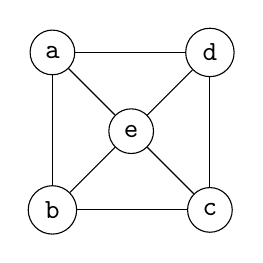
\begin{tikzpicture}
\node[draw,circle] (Na) at (0,0) {$\tta$};
\node[draw,circle] (Nd) at (2,0) {$\ttd$};
\node[draw,circle] (Ne) at (1,-1) {$\tte$};
\node[draw,circle] (Nb) at (0,-2) {$\ttb$};
\node[draw,circle] (Nc) at (2,-2) {$\ttc$};
\path[-] (Na) edge (Nd) (Na) edge (Nb) (Na) edge (Ne);
\path[-] (Nb) edge (Ne) (Ne) edge (Nd);
\path[-] (Nb) edge (Nc) (Nd) edge (Nc);
\path[-] (Ne) edge (Nc);
\end{tikzpicture}
\end{document}